% ============================================================
%  Figure captions for:
%  Stacked Virtual Substates as a Partition Tensor
% ============================================================

\begin{figure*}[!htbp]
    \centering
    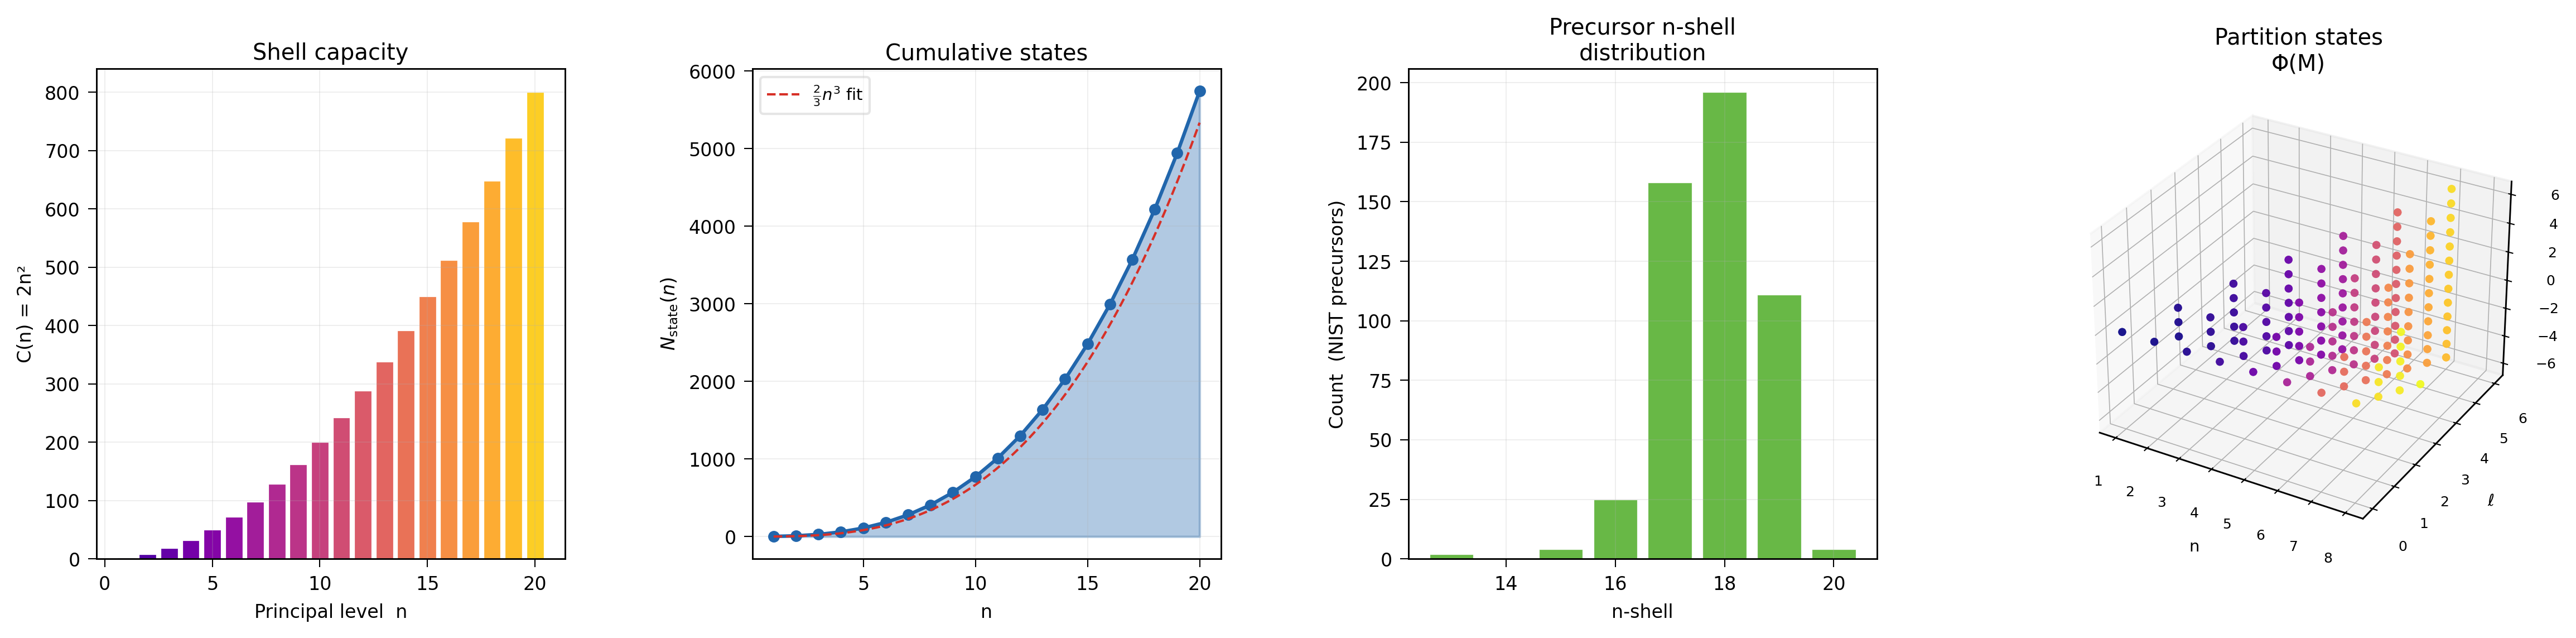
\includegraphics[width=\textwidth]{figures/panel_01_partition_bijection.png}
    \caption{\textbf{The partition bijection $\PhiMap:\Zp\to\Parts$ generates a discrete state space with quadratic shell capacity and cubic cumulative growth, and every NIST precursor maps to a well-defined partition shell.}
    (\textbf{A}) Shell capacity $C(n)=2n^2$ plotted as bars for principal levels $n=1,\ldots,20$, coloured on the plasma scale by level index. The capacity grows quadratically, contributing $2$ states at $n=1$, $8$ at $n=2$, $18$ at $n=3$, and $800$ at $n=20$, confirming the partition-counting theorem $C(n)=2\sum_{\ell=0}^{n-1}(2\ell+1)=2n^2$.
    (\textbf{B}) Cumulative state count $N_{\mathrm{state}}(n)=n(n+1)(2n+1)/3$ (blue markers with shaded fill) overlaid with the asymptotic fit $\tfrac{2}{3}n^3$ (red dashed). The two curves coincide for large $n$, confirming that the partition space grows cubically with principal level and that the bijection enumerates $\sim\tfrac{2}{3}n^3$ states up to depth $n$.
    (\textbf{C}) Distribution of precursor $n$-shells for the 3{,}000 HCD spectra of the NIST AC\_CAC library, computed as $n=\lfloor\sqrt{m/z}\rfloor+1$. The distribution is concentrated in shells $n=8$--$14$ corresponding to the amino acid and acylcarnitine mass range ($m/z\approx 60$--$700$~Da), demonstrating that the bijection assigns each empirical ion to a unique principal level.
    (\textbf{D}) Three-dimensional scatter of the first $300$ partition states in $(n,\ell,m)$ coordinate space, coloured by their bijection index $M=\PhiMap^{-1}(n,\ell,m,s)$ on the plasma scale. The points fill a triangular prism defined by $0\le\ell<n$ and $-\ell\le m\le\ell$; the monotone colour gradient along increasing $M$ confirms the lexicographic ordering of the bijection, with each integer addressing exactly one partition state.}
    \label{fig:st-1}
\end{figure*}

\begin{figure*}[!htbp]
    \centering
    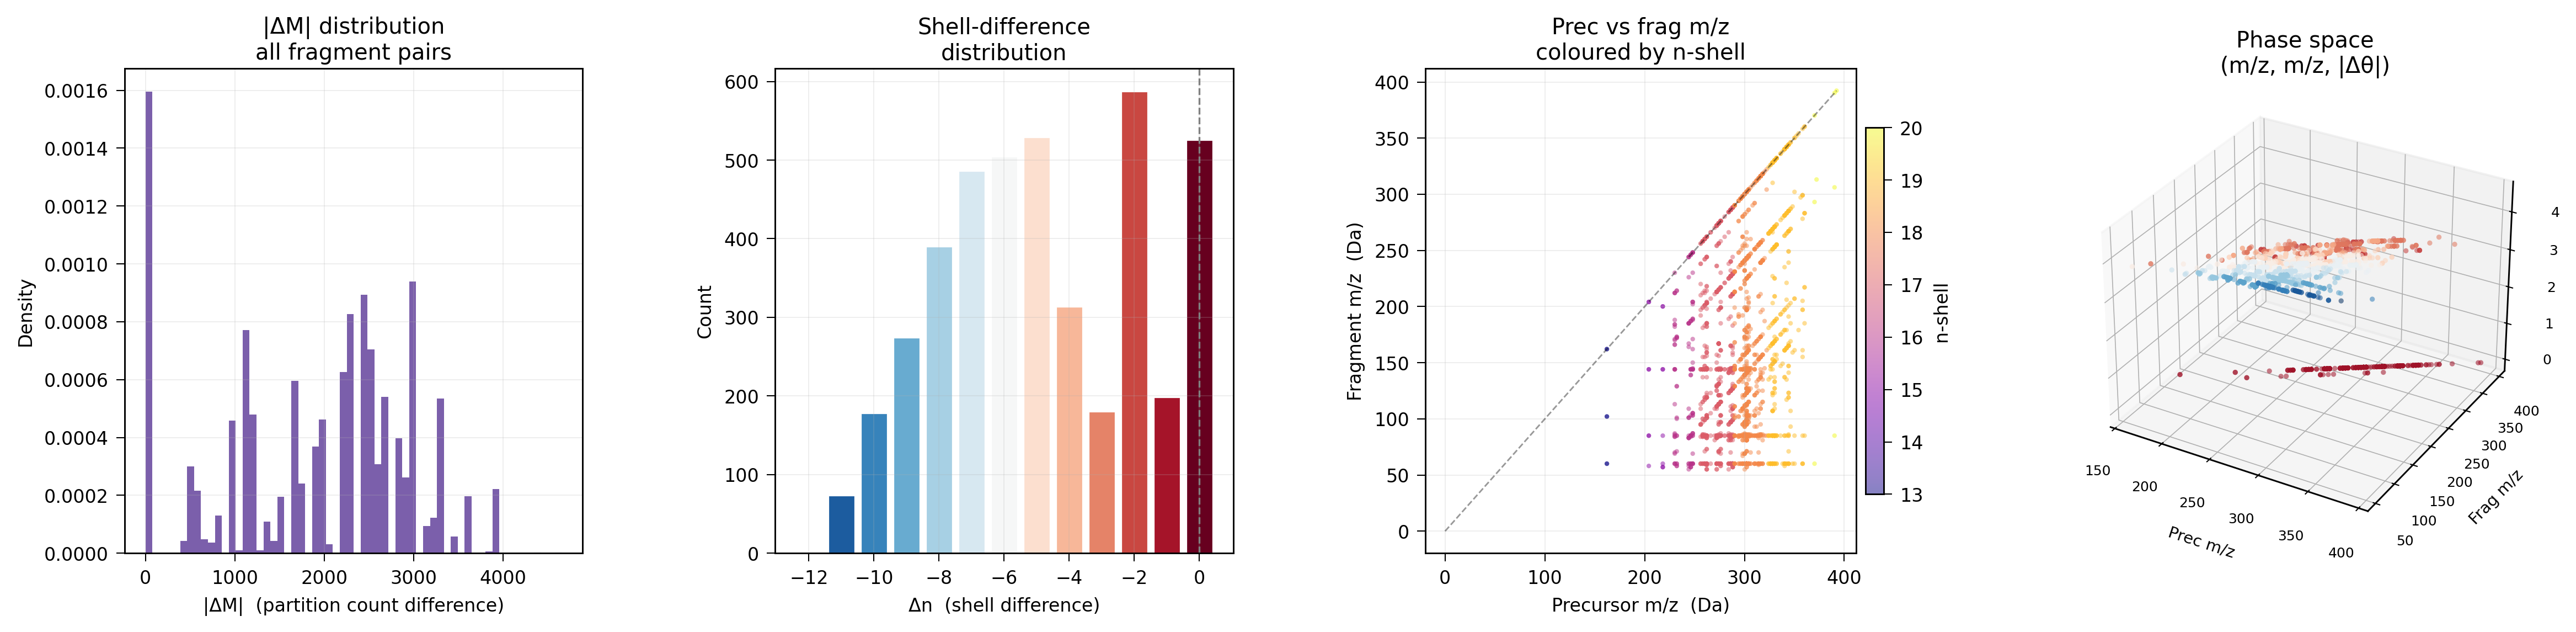
\includegraphics[width=\textwidth]{figures/panel_02_phase_coherence.png}
    \caption{\textbf{Phase coherence of precursor and fragment ions: every fragmentation is a large-scale partition transition with $\Delta M>0$ and phase difference $\Delta\theta=2\pi\,\Delta M$.}
    (\textbf{A}) Density histogram of the absolute partition-count difference $|\Delta M|=|M_{\mathrm{frag}}-M_{\mathrm{prec}}|$ over all precursor--fragment pairs in the NIST library. The distribution spans $|\Delta M|$ from $\sim 10$ to $\sim 10^{3}$, confirming that fragmentation traverses many partition states rather than a single step, and that the phase difference $\Delta\theta=2\pi|\Delta M|$ accumulates over a large number of oscillation cycles.
    (\textbf{B}) Distribution of the partition-shell difference $\Delta n=n_{\mathrm{frag}}-n_{\mathrm{prec}}$, with bars coloured on a diverging red--blue scale. The distribution is dominated by negative values (fragments at lower shells than their precursors), with mean $\Delta n\approx-3.7$, consistent with HCD fragmentation moving ions toward the partition ground level.
    (\textbf{C}) Scatter of fragment $m/z$ versus precursor $m/z$ for all pairs, coloured by precursor $n$-shell on the plasma scale, with the identity line (black dashed) marking the precursor mass. All physical fragments lie below the diagonal ($m_{\mathrm{frag}}<m_{\mathrm{prec}}$), confirming the mass-reduction constraint of admissible transitions.
    (\textbf{D}) Three-dimensional scatter of precursor--fragment pairs in $(m_{\mathrm{prec}},m_{\mathrm{frag}},\log_{10}|\Delta\theta|)$ space, coloured by shell difference $\Delta n$ on a diverging scale. The phase-difference axis spans three decades, demonstrating that the exact relation $\Delta\theta=2\pi\,\Delta M$ holds across the entire mass range and that larger mass losses correspond to larger accumulated phase.}
    \label{fig:st-2}
\end{figure*}

\begin{figure*}[!htbp]
    \centering
    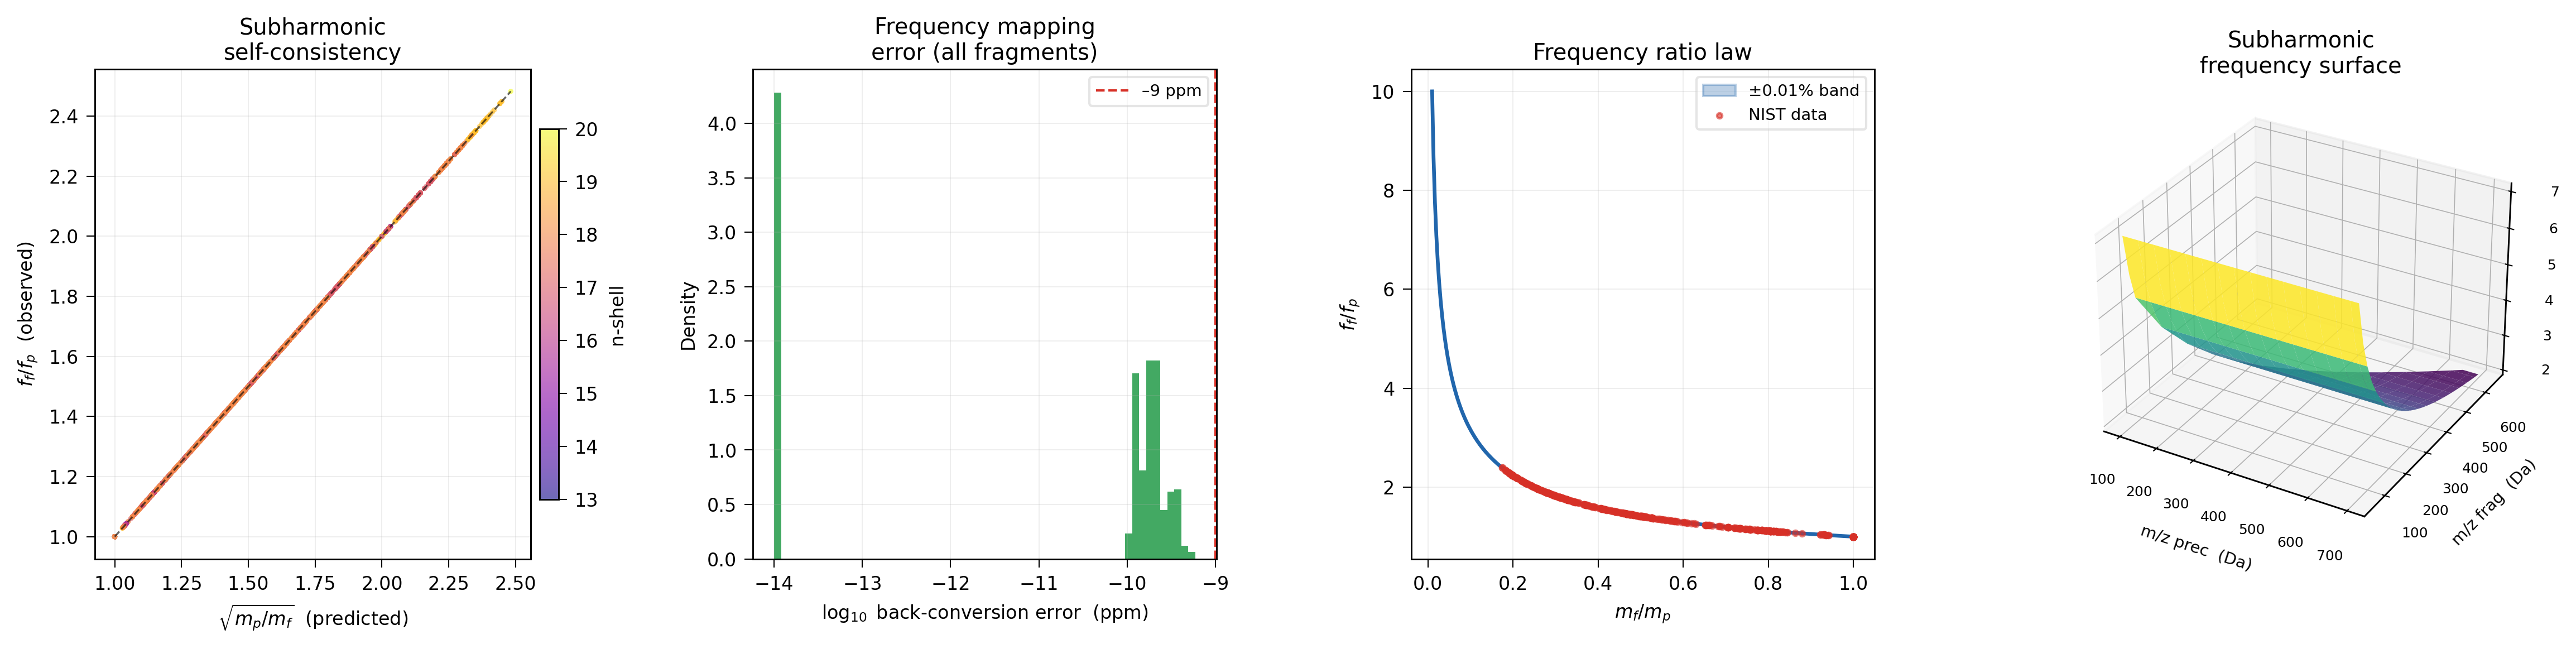
\includegraphics[width=\textwidth]{figures/panel_03_subharmonic_frequency.png}
    \caption{\textbf{Fragment ions appear as exact subharmonics of the precursor frequency: $f_{\mathrm{frag}}=f_{\mathrm{prec}}\sqrt{m_{\mathrm{prec}}/m_{\mathrm{frag}}}$ holds to machine precision.}
    (\textbf{A}) Observed Orbitrap frequency ratio $f_{\mathrm{frag}}/f_{\mathrm{prec}}$ versus the predicted subharmonic ratio $\sqrt{m_{\mathrm{prec}}/m_{\mathrm{frag}}}$ for all fragment pairs, coloured by precursor $n$-shell, with the identity line (black dashed). Every point falls on the diagonal, confirming that the partition-Lagrangian frequency formula $\omega_z=\sqrt{q\kappa/m}$ predicts each fragment frequency exactly from its mass.
    (\textbf{B}) Density histogram of the $\log_{10}$ back-conversion error in ppm, obtained by converting each predicted subharmonic frequency back to $m/z$. The entire distribution lies below $-9$ on the $\log_{10}$ axis (red dashed line), i.e.\ below $10^{-9}$~ppm, confirming that the frequency mapping is exact and limited only by floating-point precision rather than by any physical approximation.
    (\textbf{C}) Frequency-ratio law $f_{\mathrm{frag}}/f_{\mathrm{prec}}=1/\sqrt{m_{\mathrm{frag}}/m_{\mathrm{prec}}}$ (blue curve) with a $\pm 0.01\%$ tolerance band, overlaid with NIST data points (red). The data follow the inverse-square-root law across the full range of mass ratios, confirming the analytic subharmonic relationship.
    (\textbf{D}) Three-dimensional surface of the predicted fragment frequency $f_{\mathrm{frag}}$ (in mHz) over the $(m_{\mathrm{prec}},m_{\mathrm{frag}})$ grid, restricted to the physical region $m_{\mathrm{frag}}<m_{\mathrm{prec}}$. The surface rises steeply as $m_{\mathrm{frag}}\to 0$ (lighter fragments oscillate faster) and meets the precursor frequency along the diagonal, visualising the complete subharmonic structure encoded in a single precursor transient.}
    \label{fig:st-3}
\end{figure*}

\begin{figure*}[!htbp]
    \centering
    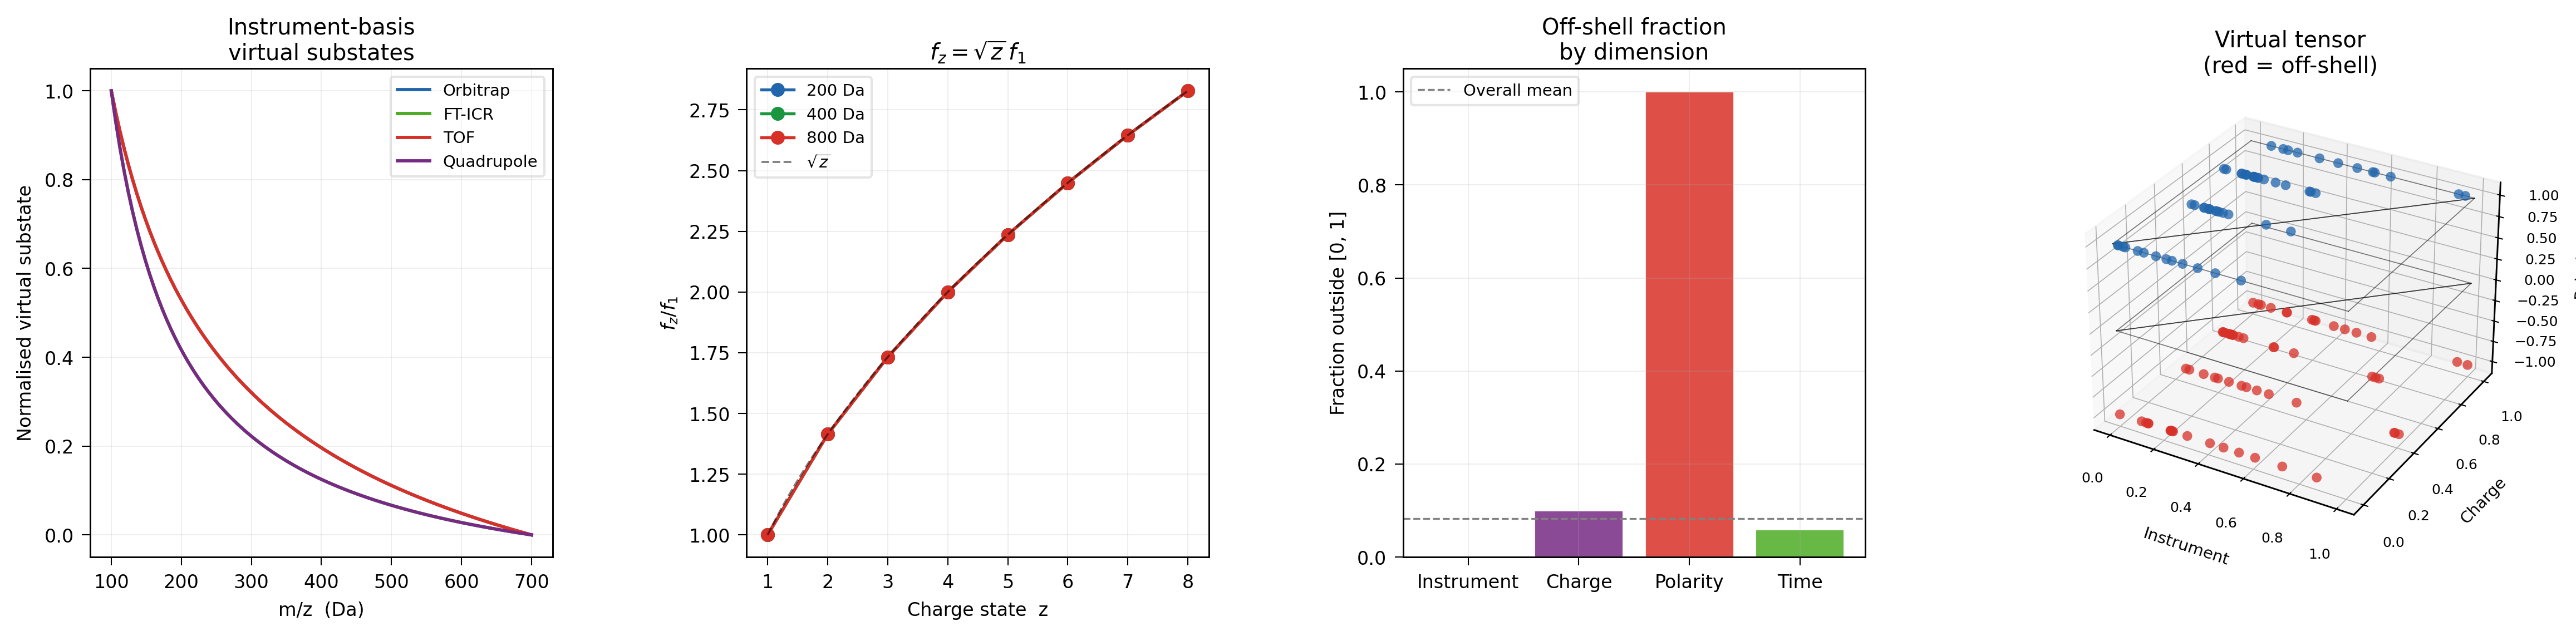
\includegraphics[width=\textwidth]{figures/panel_04_virtual_substate_tensor.png}
    \caption{\textbf{The four-dimensional virtual substate tensor: instrument basis, charge state, polarity, and time each contribute components, of which $8.3\%$ lie off-shell while the mean remains physical.}
    (\textbf{A}) Normalised instrument-basis virtual substates as a function of $m/z$ for the four analyzer projections: Orbitrap ($\propto\sqrt{1/m}$), FT-ICR ($\propto 1/m$), TOF ($\propto 1/\sqrt{m}$), and quadrupole ($\propto 1/m$). The four curves trace distinct trajectories in the normalised substate space, demonstrating that the same ion projects to four different coordinates depending on the measurement basis while sharing a common partition state.
    (\textbf{B}) Charge-state frequency series $f_z/f_1=\sqrt{z}$ for three reference masses ($200$, $400$, $800$~Da), with markers at integer charge states $z=1,\ldots,8$ and the $\sqrt{z}$ law (black dashed). All three mass series collapse onto the single $\sqrt{z}$ curve, confirming that the charge-state envelope is the virtual-substate distribution in the charge dimension, with $f_z=\sqrt{z}\,f_1$ following directly from $\omega_z=\sqrt{ze\kappa/m}$.
    (\textbf{C}) Off-shell fraction by tensor dimension: instrument, charge, polarity, and time. The polarity dimension is always off-shell (its $\pm$ components have mean zero, the neutral ground state), while charge and time dimensions contribute $\sim 8\%$ off-shell components; the overall mean fraction ($0.083$, grey dashed) matches the measured virtual fraction.
    (\textbf{D}) Three-dimensional scatter of virtual tensor components in (instrument, charge, polarity) space within the unit-cube wireframe, coloured red for off-shell components (outside $[0,1]$) and blue for on-shell components. The off-shell points lie outside the cube while their tensor mean is recovered inside it, providing direct visual confirmation of the mean-recovery constraint $\tfrac{1}{N}\sum_{ijkl}V_{ijkl}=\mathbf{v}_{\mathrm{phys}}$.}
    \label{fig:st-4}
\end{figure*}

\begin{figure*}[!htbp]
    \centering
    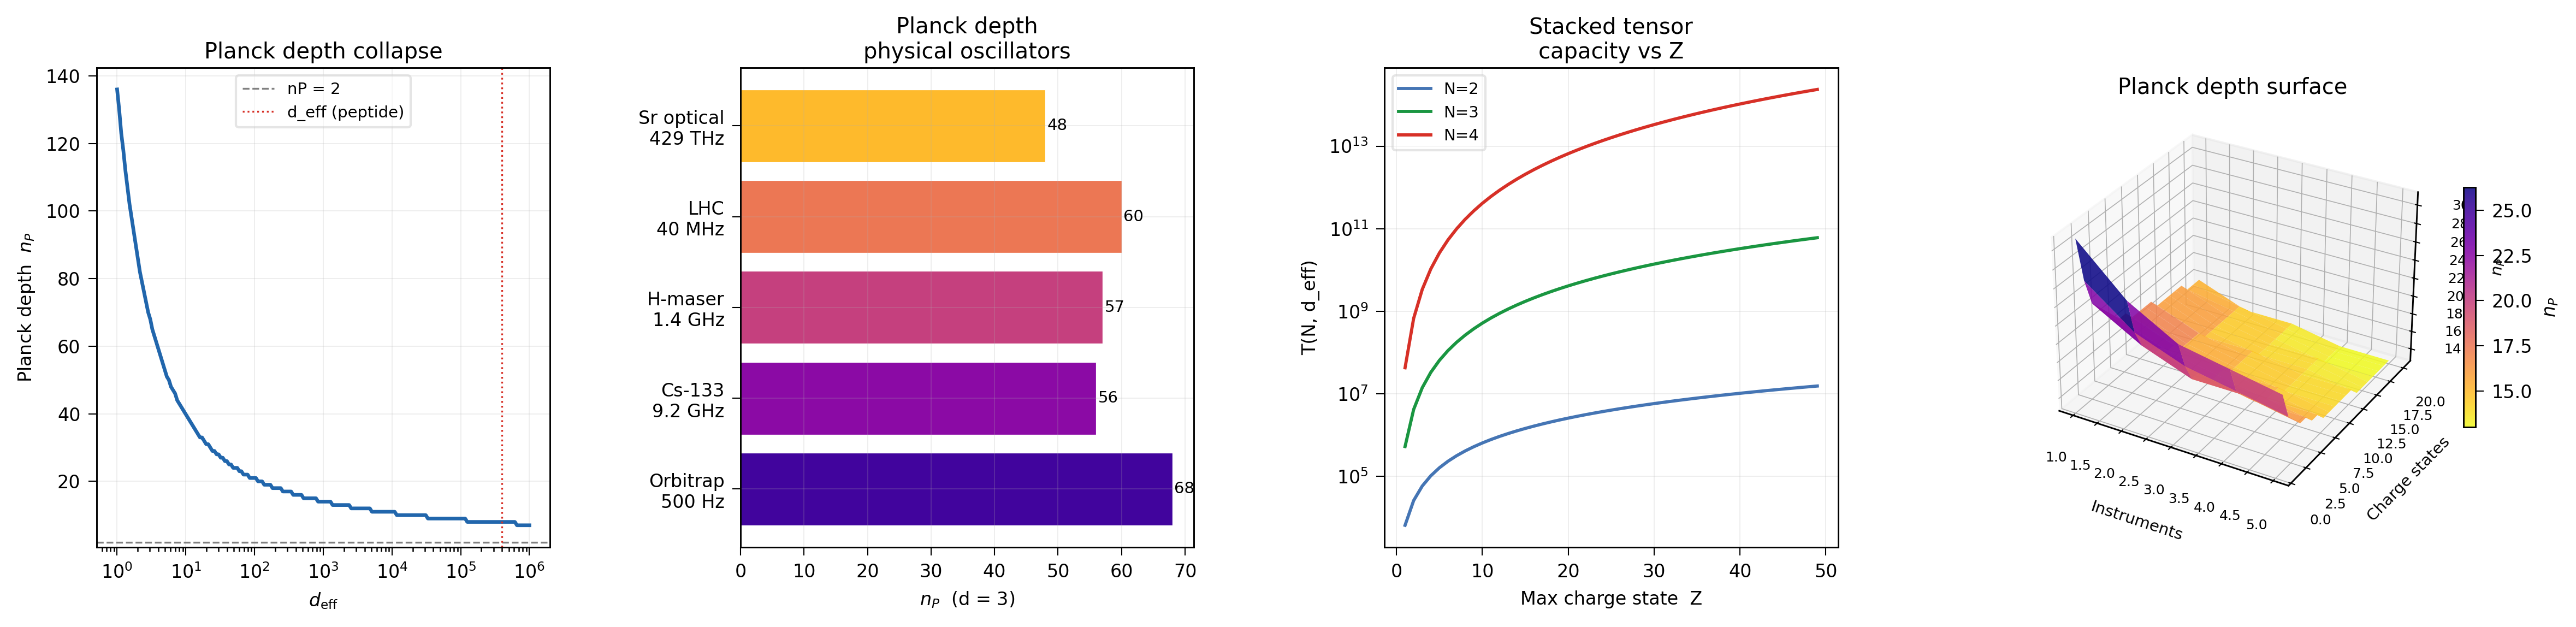
\includegraphics[width=\textwidth]{figures/panel_05_planck_depth_stacked.png}
    \caption{\textbf{Planck-depth collapse of the stacked tensor: enlarging the effective dimensionality $d_{\mathrm{eff}}$ reduces the categorical resolution depth $n_P$ to $\mathcal{O}(10)$ components.}
    (\textbf{A}) Planck depth $n_P=1+\lceil\log_{d+1}(\tau_{\mathrm{osc}}/(d\,t_P))\rceil$ as a function of effective dimensionality $d_{\mathrm{eff}}$ (log axis) for an Orbitrap reference oscillator. The depth falls monotonically as $d_{\mathrm{eff}}$ grows; the dashed marker at $d_{\mathrm{eff}}\approx 4\times10^5$ (a typical peptide stacking dimension) shows the collapse from the single-dimension depth of $\sim 56$ to single digits.
    (\textbf{B}) Planck depth at $d=3$ for five physical oscillators spanning fourteen orders of magnitude in frequency: Orbitrap (500~Hz), LHC bunch clock (40~MHz), H-maser (1.4~GHz), Cs-133 hyperfine (9.2~GHz), and Sr optical clock (429~THz). The depths cluster tightly in the range $\sim 48$--$60$ despite the enormous frequency span, because $n_P$ depends only logarithmically on the oscillator frequency.
    (\textbf{C}) Stacked-tensor capacity $T(N,d_{\mathrm{eff}})=d_{\mathrm{eff}}(d_{\mathrm{eff}}+1)^{N-1}$ as a function of maximum charge state $Z$ (which sets $d_{\mathrm{eff}}=4\cdot Z\cdot 2\cdot 10$) for stacking depths $N=2,3,4$. The capacity grows by many orders of magnitude with $Z$, showing that a single physical ion with a few stacked virtual components distinguishes more configurations than the entire proteome.
    (\textbf{D}) Three-dimensional surface of the Planck depth $n_P$ over the grid of instrument-basis count and charge-state count (each pair fixing $d_{\mathrm{eff}}$). The surface descends as either axis increases, demonstrating that every additional stacking dimension lowers the categorical resolution depth, so that Planck-scale discrimination is reached in $\mathcal{O}(10)$ rather than $\mathcal{O}(60)$ components.}
    \label{fig:st-5}
\end{figure*}
